% !TeX spellcheck = ca
% TIPUS DE DOCUMENT
\documentclass[a4paper,10pt]{article} 
% Permet canviar la mida del paper, la mida de la lletra...

% GEOMETRIA
%\usepackage[a4paper,bindingoffset=0.2in,%
%left=3cm,right=3cm,top=2.5cm,bottom=2.5cm,%
%footskip=.25in]{geometry} % Marges normals

\usepackage[a4paper,bindingoffset=0.2in,%
left=1in,right=1in,top=1in,bottom=1in,%
footskip=.25in]{geometry} % Marges estrets

% IDIOMA 
%\usepackage[catalan]{babel} %Fa que l'idioma del document sigui en català (p.ex. escriurà "Resum" enlloc de "Abstract")
\usepackage[english]{babel} %Fa que l'idioma del document sigui l'anglès

% ENCODING
\usepackage{cmap,lmodern}  % Útil tenir-ho sempre.
\usepackage[T1]{fontenc} % Millora els caràcters del pdf que es produeix
\usepackage[utf8]{inputenc} % Evita problemes amb què LaTeX no sàpiga llegir certs caràcters.
\usepackage{hyperref} % Permet que els links siguin clicables en lectors pdf

% IMATGES
% \usepackage{wrapfig,graphicx} % Permet afegir imatges
%\graphicspath{{Imatges/} % Si volem guardar totes les imatges en una carpeta (+ còmode)
\usepackage[font=small]{caption} % Peus de foto
% \usepackage{subcaption} % Subpeus de foto
% \usepackage{tikz}
% \usepackage{float}
% \usepackage{pgfplots}
% \usepackage{multirow}
\usepackage[labelfont=bf]{caption}
\usepackage{fancyhdr}
\usepackage{bm}
\usepackage{hyperref}
\usepackage{graphicx}
% \usepackage{gensymb}
\usepackage{amsmath}
\usepackage{amssymb}
% \usepackage{siunitx}
\usepackage{parskip}
% \usepackage{blindtext}
\usepackage{graphicx}
\usepackage[utf8]{inputenc}
% \usepackage{multirow}
\usepackage{longtable}
\usepackage{fancyvrb}
\usepackage{xcolor}
\usepackage{subcaption}
\usepackage{wrapfig}
\usepackage{fancyhdr}
	
% EQUACIONS
% \usepackage{mathtools,amsmath,amssymb,systeme,braket} % Diverses eines d'equacions
	
% OTROS
\setlength{\parindent}{0em}   % Controla la indentació de la primera línia de cada paràgraf
%\setlength{\parskip}{0.3em}   % Controla la mida de 'espaiat entre paràgrafs
%\usepackage{enumitem} %Permet el control sobre llistes
%\setlist{noitemsep,nolistsep} % Controla l'espaiat entre elements de llista (requereix el paquet enumitem)
	
\usepackage{fancyhdr}
\usepackage{tcolorbox}% TIPUS DE DOCUMENT
	
\pagestyle{fancy}
\fancyhf{}
\rhead{Aina Gaya}
\lhead{Pràctiques de models QM i MM}
\cfoot{\thepage}
	%
	%opening
\title{\textsc{{\large Molecular modelling } \\ Analysis of properties of a Lennard-Jones liquid } \\  {\small Molecular Dynamics}}
\author{Aina Gaya Àvila \\ {\small Lecturer: Carles Calero }}
	
\begin{document}
		
\maketitle

\section{Introduction: Molecular Dynamics Simulations code}
\subsection{A system of N particles interacting through a Lennard-Jones potential in contact with a heat bath} 

El model microscòpic més senzill per simular una substància capaç d'existir tant en estat sòlid, líquid com gasós està basat en partícules esfèriques que interactuen entre elles. Aquesta interacció es modelitza tenint en compte dues característiques:
\begin{itemize}
	\item La resistència a la compressió, és a dir, que cada partícula ocupa el seu espai i a curt abast la interacció és repulsiva. És el principi d'exclusió de Pauli.
	\item Les forces de Van der Waals entre àtoms als estats sòlid i líquid, que tendeixen a apropar les partícules.
\end{itemize}

El potencial més emprat per simular el descrit anteriorment és el de Lennard-Jones. Per descriure el potencial entre dues particules $i$ i $j$, localitzades a $r_i$ i $r_j$, pren la forma següent:

$$ u(r_{ij}) = 4 \epsilon \left[ \left( \frac{\sigma}{r_{ij}}\right)^{12} - \left( \frac{\sigma}{r_{ij}}\right)^{6} \right] $$

On 

\begin{itemize}
	\item $r_{ij} = | r_i - r_j | $ és la distància entre partícules.
	\item $\sigma$ defineix la mida de la partícula.
	\item $\epsilon$ és la profunditat del potencial. És una mesura de la magnitud de la interacció.
\end{itemize}

The main goal of this project is to do a computer simulation of a Lennard-Jones liquid in order to be able to study its properties.

A Lennard-Jones liquid is characterized by 2 parameters: $\epsilon$ and $\sigma$. 

\begin{figure}
	\centering
	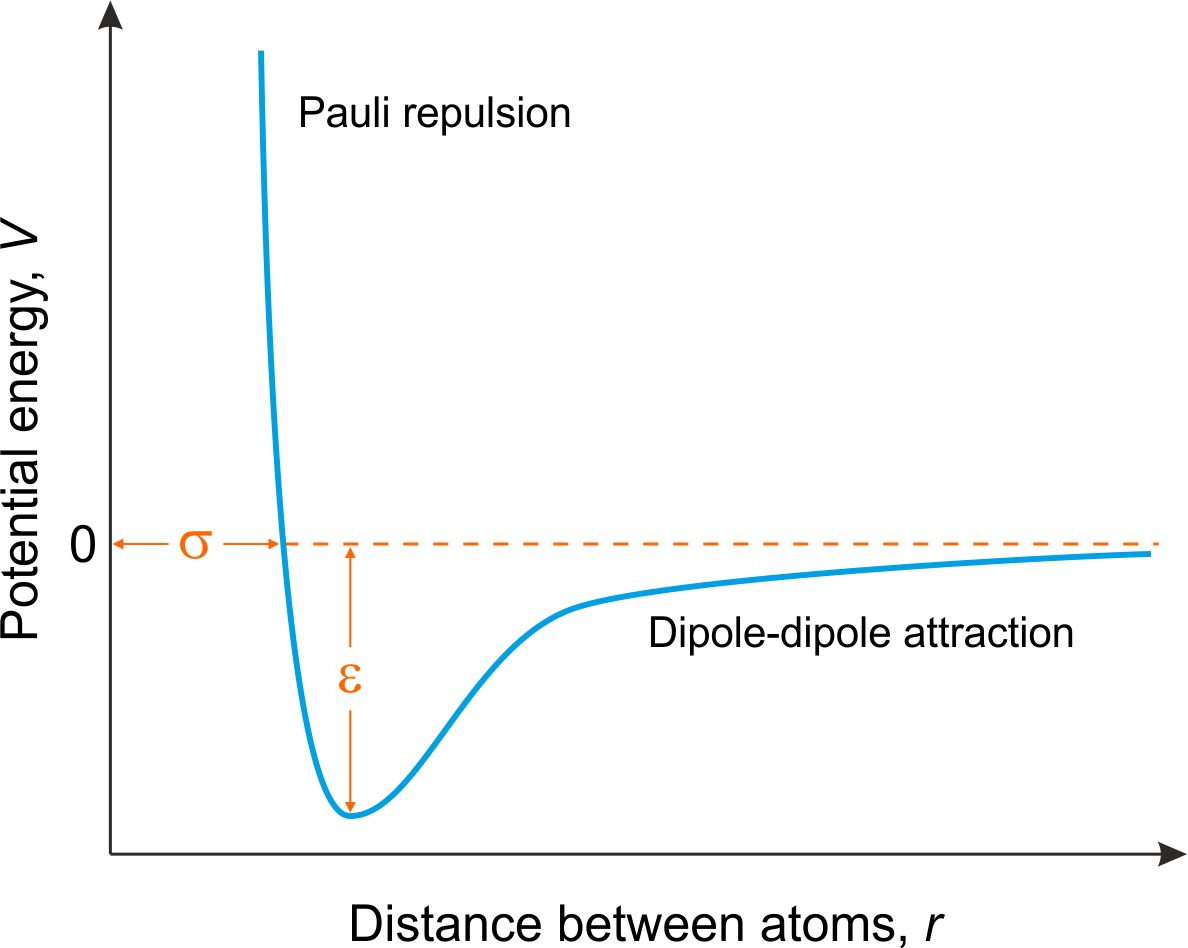
\includegraphics[width=0.7\linewidth]{lennard-jones_potential}
	\caption{A Lennard-Jones potential.}
	\label{fig:lennard-jonespotential}
\end{figure}


%(a) Describe in detail the different parts of the code. How do you initialize the system of particles (and set the density)? What integrator do you use? How do you implement periodic boundary conditions? How do you control the temperature (how do you implement the thermostat)? What units do you use for the Lennard-Jones interactions? What cut-off do you use for the interactions (and why)? What truncation strategy do you choose?

The system is inicialized using a simple cubic structure. The desity is fixed in $\rho = 0.7 m\sigma^3$. 

\end{document}